% Created 2016-08-17 Wed 14:38
\documentclass[tikz,12pt]{standalone}

\usepackage[utf8]{inputenc}
\usepackage[T1]{fontenc}
\usepackage{helvet}
\usepackage{../../templates/msc}

\renewcommand{\familydefault}{\sfdefault}

\tikzset{
every picture/.style={
line width=1pt
}}

\usepackage{tikz}
\author{Holger Karl}
\date{\today}
\title{}

\usetikzlibrary{decorations.pathreplacing}

\usepackage{marvosym}
\usepackage{calc}



\begin{document}

    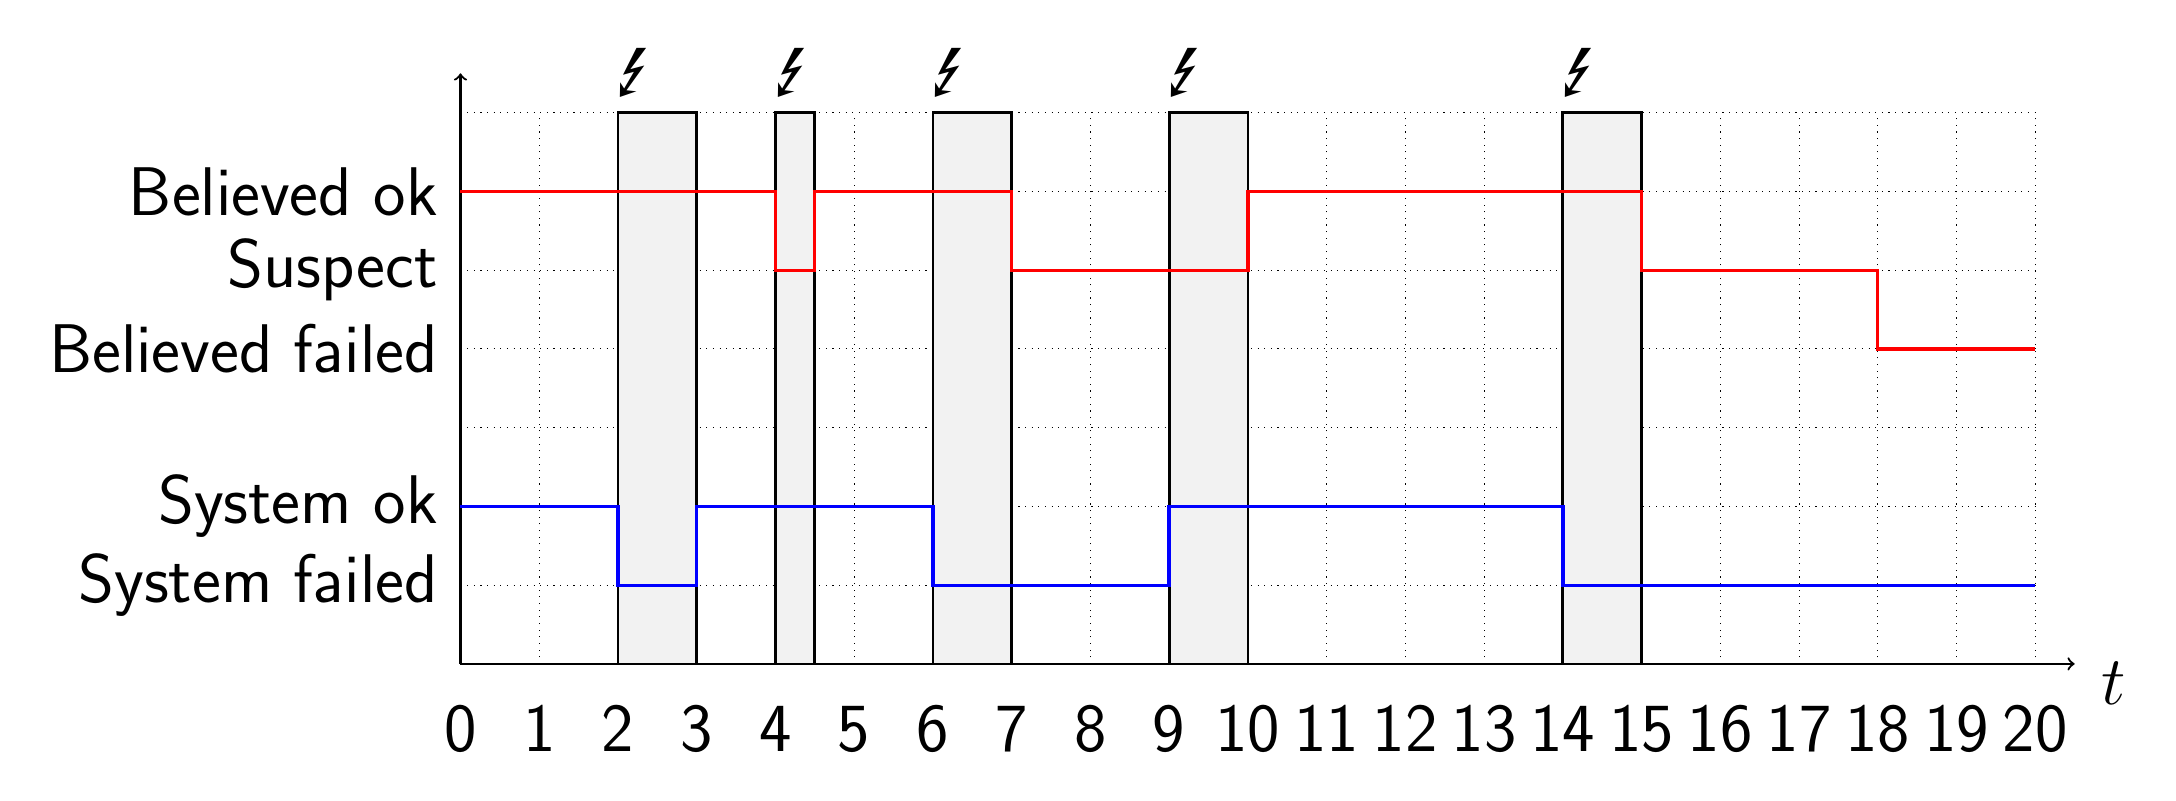
\begin{tikzpicture}
      \Huge

      % grid and coordinates: 
      \draw [dotted, thin ] (0,0) grid (20, 7);
      \draw [thick, ->] (0,0) -- (20.5, 0); 
      \draw [thick, ->] (0,0) -- (0, 7.5); 
      \node at (21, -0.25) {$t$}; 
      \foreach \x in {0,1, ..., 20}  \node[anchor=north] at (\x,-0.25) {\x};
      % system and detector states: 
      \node[anchor=east] (left) at (0, 6) {Believed  ok}; 
      \node[anchor=east] (left) at (0, 5) {Suspect}; 
      \node[anchor=east] (left) at (0, 4) {Believed  failed}; 

      \node[anchor=east] (center) at (0, 2) {System ok}; 
      \node[anchor=east] (right) at (0, 1)  {System failed}; 

      % time frames of discrepancies: 
      \foreach \s/\e in {2/3, 4/4.5,6/7,9/10,14/15}  {
        \draw[fill=gray!10] (\s,0) rectangle (\e,7);  
        \node at (\s+0.2,7.5) {\Huge\Lightning}; 
        % This is what I really want: 
        % \node at (0.5\s+0.5\e,7.5) {\Huge\Lightning}; 
      }

      % \draw[fill=gray!10] (2,0) rectangle (3,7);    \node at (2.5,7.5) {\Huge\Lightning}; 
      % \draw[fill=gray!10] (4,0) rectangle (4.5,7); \node at (4.25,7.5) {\Huge\Lightning};


      % system ground truth: 
      \draw [very thick, blue] (0,2) -- (2,2) -- (2,1) -- (3, 1) -- (3,2)
      -- (6,2) -- (6, 1) -- (9, 1) -- (9, 2) -- (14, 2) -- (14, 1) --
      (20,1); 
      
      % detector: 
      \draw[very thick, red] (0, 6) -- (4,6) -- (4, 5) -- (4.5, 5) --
      (4.5, 6)  -- (7,6) --  (7,5) -- (10,5) -- (10,6) -- (15, 6) --
      (15, 5) -- (18,5) -- (18,4) -- (20, 4); 

    \end{tikzpicture}

\end{document}